\documentclass{article}

\usepackage{url}
\usepackage{fancyhdr}
\usepackage{extramarks}
\usepackage{amsmath}
\usepackage{amsthm}
\usepackage{amsfonts}
\usepackage{tikz}
\usetikzlibrary{3d}
\usepackage[plain]{algorithm}
\usepackage{algpseudocode}
\usepackage{braket}
\usepackage{enumerate}
\usepackage{paralist}
\usepackage{listings}
%
% Basic Document Settings
%

\topmargin=-0.45in
\evensidemargin=0in
\oddsidemargin=0in
\textwidth=6.5in
\textheight=9.0in
\headsep=0.25in

\linespread{1.1}

\pagestyle{fancy}
\lhead{Habib University}
\chead{\hmwkClass, \hmwkTitle}
\rhead{\firstxmark}
\lfoot{\lastxmark}
\cfoot{\thepage}

\renewcommand\headrulewidth{0.4pt}
\renewcommand\footrulewidth{0.4pt}

\setlength\parindent{0pt}

\definecolor{mGreen}{rgb}{0,0.6,0}
\definecolor{mGray}{rgb}{0.5,0.5,0.5}
\definecolor{mPurple}{rgb}{0.58,0,0.82}
\definecolor{backgroundColour}{rgb}{0.95,0.95,0.92}

\lstdefinestyle{CStyle}{
    backgroundcolor=\color{backgroundColour},
    commentstyle=\color{mGreen},
    keywordstyle=\color{magenta},
    numberstyle=\tiny\color{mGray},
    stringstyle=\color{mPurple},
    basicstyle=\footnotesize,
    breakatwhitespace=false,
    breaklines=true,
    captionpos=b,
    keepspaces=true,
    numbers=left,
    numbersep=5pt,
    showspaces=false,
    showstringspaces=false,
    showtabs=false,
    tabsize=2,
    language=C
}

%
% Create Problem Sections
%

\newcommand{\enterProblemHeader}[1]{
	\nobreak\extramarks{}{Problem \arabic{#1} continued on next page\ldots}\nobreak{}
	\nobreak\extramarks{Problem \arabic{#1} (continued)}{Problem \arabic{#1} continued on next page\ldots}\nobreak{}
}

\newcommand{\exitProblemHeader}[1]{
	\nobreak\extramarks{Problem \arabic{#1} (continued)}{Problem \arabic{#1} continued on next page\ldots}\nobreak{}
	\stepcounter{#1}
	\nobreak\extramarks{Problem \arabic{#1}}{}\nobreak{}
}

\setcounter{secnumdepth}{0}
\newcounter{partCounter}
\newcounter{homeworkProblemCounter}
\setcounter{homeworkProblemCounter}{1}
\nobreak\extramarks{Problem \arabic{homeworkProblemCounter}}{}\nobreak{}

%
% Homework Problem Environment
%
% This environment takes an optional argument. When given, it will adjust the
% problem counter. This is useful for when the problems given for your
% assignment aren't sequential. See the last 3 problems of this template for an
% example.
%
\newenvironment{homeworkProblem}[1][-1]{
	\ifnum#1>0
	\setcounter{homeworkProblemCounter}{#1}
	\fi
	\section{Problem \arabic{homeworkProblemCounter}}
	\setcounter{partCounter}{1}
	\enterProblemHeader{homeworkProblemCounter}
}{
	\exitProblemHeader{homeworkProblemCounter}
}

%
% Homework Details
%   - Title
%   - Due date
%   - Class
%   - Section/Time
%   - Instructor
%   - Author
%

\newcommand{\hmwkTitle}{Assignment\ \#2}
\newcommand{\hmwkDueDate}{February 10, 2024, 11.59pm}
\newcommand{\hmwkClass}{CS 201 - Data Structures and Algorithms II}
\newcommand{\hmwkClassInstructor}{Muhammad Mobeen Movania (L1),\\ Syeda Saleha Raza (L2),\\ Faisal Alvi (L3, L4),\\ Abdullah Zafar (L5).}
\newcommand{\hmwkAuthorName}{\textbf{Student 1 Name, ID} \and \textbf{Student 2 Name, ID}}

%
% Title Page
%

\title{
	\vspace{2in}
	\textmd{\textbf{\hmwkClass:\\ \hmwkTitle}}\\
	\normalsize\vspace{0.1in}\small{\hmwkClassInstructor}\\
	\normalsize\vspace{0.1in}\small{Due\ on\ \hmwkDueDate}\\
	\vspace{3in}
}

\author{\hmwkAuthorName}
\date{}

\renewcommand{\part}[1]{\textbf{\large Part \Alph{partCounter}}\stepcounter{partCounter}\\}

%
% Various Helper Commands
%

% Useful for algorithms
\newcommand{\alg}[1]{\textsc{\bfseries \footnotesize #1}}

% For derivatives
\newcommand{\deriv}[1]{\frac{\mathrm{d}}{\mathrm{d}x} (#1)}

% For partial derivatives
\newcommand{\pderiv}[2]{\frac{\partial}{\partial #1} (#2)}

% Integral dx
\newcommand{\dx}{\mathrm{d}x}

% Alias for the Solution section header
\newcommand{\solution}{\textbf{\large Solution}}

% Probability commands: Expectation, Variance, Covariance, Bias
\newcommand{\E}{\mathrm{E}}
\newcommand{\Var}{\mathrm{Var}}
\newcommand{\Cov}{\mathrm{Cov}}
\newcommand{\Bias}{\mathrm{Bias}}

\begin{document}
	
\maketitle
	
\pagebreak
\section{Instructions}
This assignment document consists of two problems.

\begin{itemize} 
	\item \underline{Problem 1} is a theoretical question which requires analysis. It should be completed and submitted within this document. This problem is worth 20 points.
	\item \underline{Problem 2} is a programming based question which requires implementation. It must be submitted as a zipped archive containing:
\begin{enumerate}
	\item your programs (the language of implementation in C++), 
	\item the input files provided to you, and
	\item the output files generated by your program. 
\end{enumerate}

The solution to program 2 will be graded for correctness and structure by testing the output against test input files. This problem is worth 40 points.

\end{itemize}
\newpage
\begin{homeworkProblem}
(20 points) [\textbf{Amortized Analysis}] Let us define a \texttt{stop-min-stack} with a stack as the underlying data structure, which stores a sequence of items and has the following operations:
\begin{enumerate}
	\item \texttt{push(\textit{x})} adds the item \texttt{\textit{x}} to the top of the underlying stack.
	\item \texttt{peek()} returns the item at the top of the underlying stack without removing it.
	\item \texttt{stop-min-pop()} pops a local minimum from the existing items in the stack. This operation works as follows:
	\begin{enumerate}[(a)]
		\item removes an existing item from the stack using \texttt{pop()}, (if the stack was empty before the \texttt{pop()}, NULL is returned; if the stack is empty as a result of the \texttt{pop()}, the popped item is returned) 
		\item tests whether the popped item is greater than or equal to the current item at the top of the underlying stack using \texttt{peek()}. 
		\item If yes, the recently popped item is discarded. 
		\item Steps (a) - (c) are repeated as a loop until the recently popped item is less than the topmost item in the stack or if the underlying stack is empty. 
		\item Finally, the recently popped item is returned.
	\end{enumerate}
\end{enumerate}
For example if the stack contains the items 4, 3, 2, 9, 5, then after one application of \texttt{stop-min-pop()}, the item 2 will be returned and the stack will have the elements 9, 5 as shown below:
% Please add the following required packages to your document preamble:
% \usepackage{graphicx}

\begin{table}[h]
	\centering
	\begin{tabular}{|c|c|c|}
			4 &  &   \\ \cline{1-1}
			3 &  &   \\ \cline{1-1}
			2 &  &   \\ \cline{1-1} \cline{3-3} 
			9 &  & 9 \\ \cline{1-1} \cline{3-3} 
			5 &  & 5 \\ \cline{1-1} \cline{3-3} 
		\end{tabular}%
	\caption{\texttt{Stop-min-stack} before and after one application of \texttt{stop-min-pop()}}
\end{table}

%%\begin{figure} [H]
%% 	\centering
%% 	\includegraphics[scale = 0.7]{bell-states.png}
%% 	\caption{The Four Bell States $\ket{\phi^+}$, %%$\ket{\phi^-}$, $\ket{\psi^+}$, $\ket{\psi^-}$}
%%\end{figure}
		
\begin{enumerate}[(a)]
\item (5 points) Using an underlying Stack which has only \texttt{push}, \texttt{pop} and \texttt{peek} as its operations with constant time complexity, write pseudocode for the operation \texttt{stop-min-pop()}. What is the time complexity of \texttt{stop-min-pop()} in the worst case for a stack of size $n$? 
\item (5 points) Give an argument using worst case analysis that if \texttt{stop-min-pop()} is applied $n$ times to an arbitrary stack of size $n$, the worst case time complexity can be O$(n^2)$, thereby giving a cost of O$(n)$ per operation.

\item (10 points) Using amortized analysis, show that the amortized cost of applying \texttt{stop-min-pop()} $n$ times to an arbitrary stack of size $n$ is actually O(1) per operation.
\end{enumerate}

\end{homeworkProblem}
\bigskip

\newpage
\begin{homeworkProblem} (40 points) [\textbf{Optimizing particle-particle collisions through spatial hashing.}] 

You will apply the knowledge of hashing to implement spatial hashing to resolve particle-particle collisions \cite{ref1} as shown in Figure \ref{fig3}. Template code has been shared with you which implements particle particle collisions through brute force method. However, the spatial hashing code does not implement spatial hashing for collision detection between particles. You can press 'h' key to toggle from using spatial hashing (default) to brute force method. As you would expect, the frame rate grinds down to a halt when brute force method is used. 

\begin{figure}
\centering
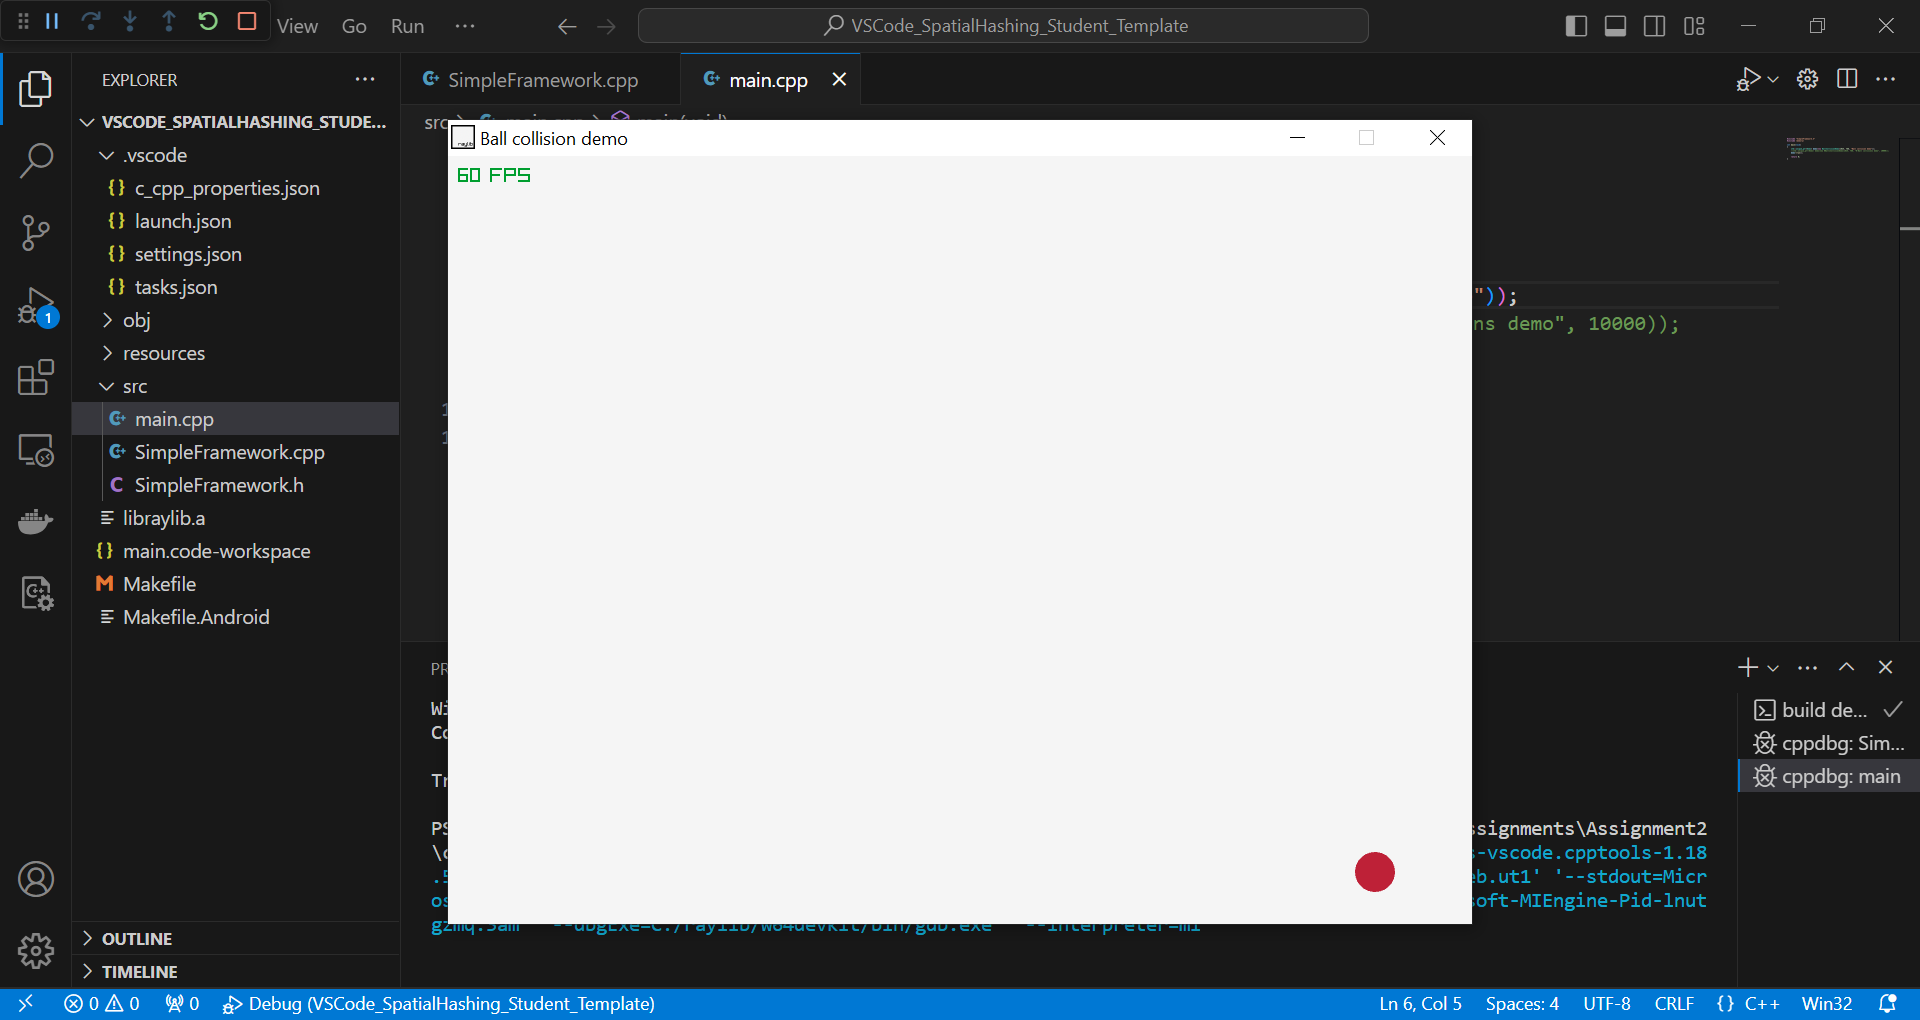
\includegraphics[width=0.9\textwidth]{fig/fig3}
\caption{N-particles collision demo with 100 particles.}
\label{fig3}
\end{figure}

For this assignment, you need to add collision detection in the shared template code using spatial hashing. You can get the technical overview of the method using reference \cite{ref1} and a more implementation friendly description is shared in reference \cite{ref2}.  Relevant sections of the code are marked with TODOs so you can know where you need to add additional code.  

If you have implemented spatial hashing based collision correctly, you should see collision detection and response happening at interactive framerates unlike the brute force method which makes the application unusable. Moreover, the UI should display the total collisions detected on screen which in the default template should be 0.

\subsection{Setting up raylib}
The basic skeleton code is built on top of raylib \cite{ref3}. You should be able to clone the assignment2 github repository and open the folder in VSCode. It should compile out of the box. If you want to get some details on the installation of raylib, the steps to install raylib are given for all platforms separately. For Windows OS, they are given here: \url{https://github.com/raysan5/raylib/wiki/Working-on-Windows}. For other OS, refer to \url{https://github.com/raysan5/raylib}.  Note for the given code, there is no additional step required. All setup is done already for you. For those of you working on non-Windows OSes, you may refer to the raylib installation steps or get connected with one of the course TAs.

\subsection{Running the template code}
Go to VSCode and open the template code folder. Press F5 or go to \textbf{Run menu} and then select \textbf{Start Debugging}. If all goes well, your should see the application run as shown in Figure \ref{fig1}. By default, the code uses spatial hashing with boundary collisions but it does not implement particle-particle collision. The brute force method does the collision both with the boundaries as well as with all other particles. You can press 'h' key to toggle using spatial hashing to use brute force method. Note that the performance of the application will slow down considerably if you use the brute force method for collision detection.

\begin{figure}
\centering
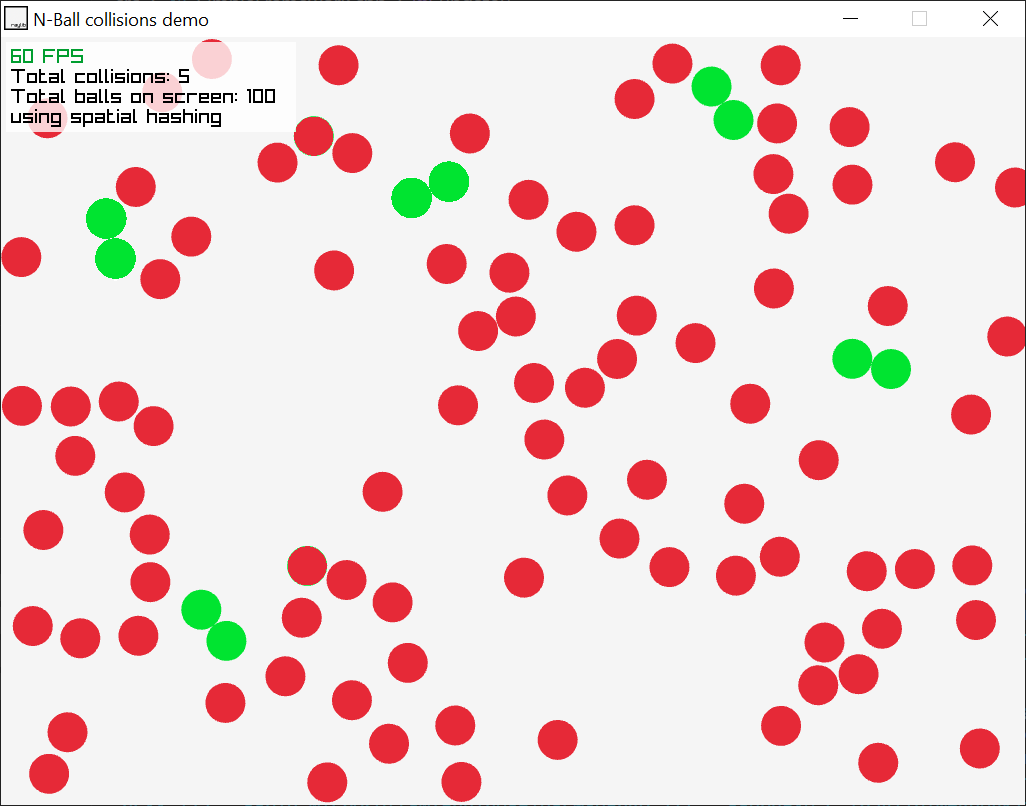
\includegraphics[width=\textwidth]{fig/fig1}
\caption{Running the template code.}
\label{fig1}
\end{figure}

\subsection{Template code framework details}
The C++ template code uses a fairly simple C++ framework. There is a base class called \textbf{Demo}. This class sets up raylib and the event loop so that you do not have to repeat the steps in your own application. There are four pure virtual functions in the Demo class which are detailed as in Listing \ref{list1}.

\begin{lstlisting}[language=C++, caption={Demo class pure virtual functions.}, label={list1}, style=CStyle]
virtual void init() = 0;
virtual void shutdown() = 0;
virtual void draw() = 0;
virtual void update() = 0;
\end{lstlisting}
The init function is where you would do initialization of your application data structures and other variables. The shutdown method will do the de-initialization that is removing every data structure and data that you will use in your application. The draw function will be where the displaying of the objects will take place and finally, the update function is where the physics simulation will be updated.  

\subsection{Simple particle collision demo}
Within the template framework code, we have given a simple example class inheriting from the \texttt{Demo} class called \texttt{BallCollisionDemo}. This class implements a single particle moving in the window and colliding with the screen bounds. You can see how we override the virtual methods of the \texttt{Demo} class.  This is given as a simple example for you to help understand the given \texttt{Demo} framework structure. In order to run this demo, please uncomment line 6 and comment line 7 of main.cpp and then press 'F5' or go to \textbf{Run menu} and then \textbf{Start Debugging}. If all goes well, you should see a single particle moving in the screen and colliding with the screen bounds as shown in Figure \ref{fig2}. Note that the \texttt{BallCollisionDemo} is for your understanding only. You will implement spatial hashing in \texttt{NBallsCollisionDemo}.

\begin{figure}
\centering
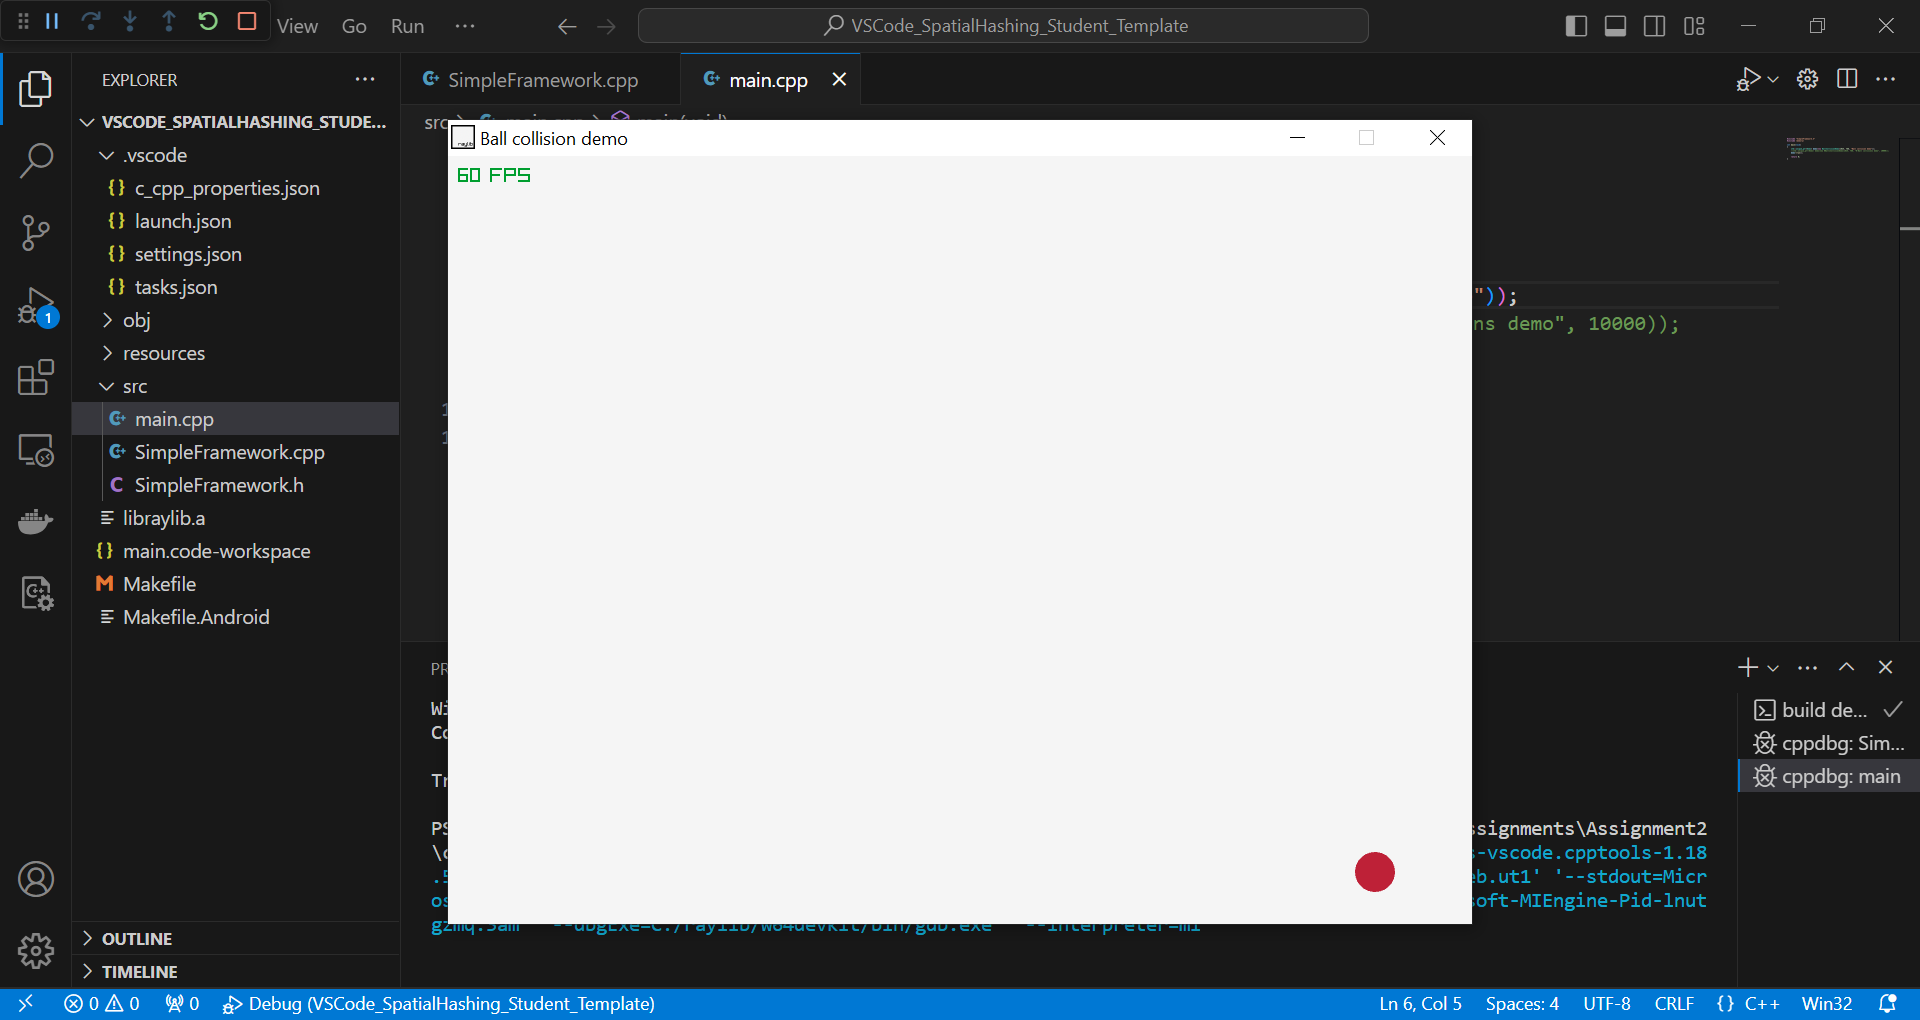
\includegraphics[width=\textwidth]{fig/fig2}
\caption{Simple particle demo example.}
\label{fig2}
\end{figure}

\subsection{N particles collision demo}
Within the template framework code, we provide another example class inheriting fom the \texttt{Demo} class called \texttt{NBallsCollisionDemo}. This class implements 10000 particles moving in the window and colliding with the screen bounds. All of the code for initialization and handling of rendering of the 10000 particles is already taken care of for you. In addition, the basic screen collision is also implemented. We provide the brute force inter particle collision code, see lines 187-228 \texttt{SimpleFramework.cpp} but the spatial hashing based optimized inter particle collision detection is missing and this is what you are required to implement in the given framework. 

For your assistance, the relevant sections of the code are marked with TODOs comments so you can add relevant code there. Please note that you are free to add code any where you deem fit but please do not remove the code that is already provided. For testing, you can change the last parameter of the NBallsCollisionDemo constructor call in main.cpp to 100 to reduce the total number of particles on screen. This will help you debug the code faster. Once you are fine with the code, dont forget to change the last parameter back to 10000.

\subsection{Required Tasks}
You should implement a C++ class Hash that should contain all necessary data structures and functions. You should provide at least two functions: a function to repopulate the hash grid given all particle positions and another function to return the list of particles in the hash grid where the given particle position hashes to. 

\vspace{0.5cm}

\textbf{Rubric:} Your submission will be evaluated on the following rubric. Your C++  \texttt{Hash} class should:
\begin{itemize}
\item (15 points) implement spatial hashing using appropriate data structures, 
\item (10 points) provide correct output for different configration of particle count and particle radii (Note that all particles will have the same radii.), 
\item (10 points) provide necessary functions to accelerate the neighbor search 
\item (5 points) use proper naming convention with well commented code.
\end{itemize}
\end{homeworkProblem}

We are providing you with two folders: \texttt{input} containing input files and \texttt{output} containing the corresponding simplified output files. Your program should read in every input file in the input folder and produce the corresponding output files in a folder called "test-output".
\\

Further submission guidelines will be provided to you later.
\\

Due date: Sunday, 10 March 2024, 11.59pm.

\begin{thebibliography}{9}
\bibitem{ref1} 
Matthias Teschner, Bruno Heidelberger, Matthias Muller, Danat Pomeranets, and Markus Gross, \textit{"Optimized Spatial Hashing for Collision Detection of Deformable Objects"}, in Proceedings of the 8th Workshop on Vision, Modeling, and Visualization (VMV 2003), Munich, Germany, 2003.

\bibitem{ref2}
Blogpost: The mind of Conkerjo, \textit{Spatial hashing implementation for fast 2D collisions}, available online: https://conkerjo.wordpress.com/2009/06/13/spatial-hashing-implementation-for-fast-2d-collisions/

\bibitem{ref3}
Ramon Santamaria (@raysan5), {raylib: a simple and easy-to-use library to enjoy videogames programming}, available online: https://www.raylib.com/
 
\end{thebibliography}

\end{document}

